\chapter{Contractual}

It is important that all Engineers are aware of the original scope of works. The original scope of works can be found here.

Responsibility for raising the issue of V.O.'s is as follows:

\begin{figure}
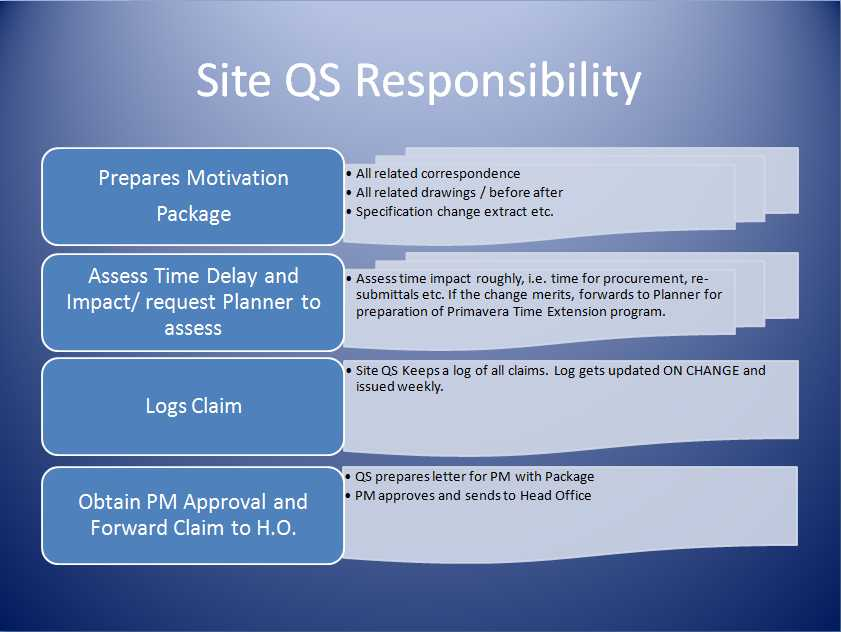
\includegraphics[width=1.3\textwidth]{./graphics/Site-QS-responsibilities}
\end{figure}


It is a very rare occassion that the person originating the change will
issue an instruction and a variation without us asking for it. However,
small this request is, being professional and recording the change will
ensure that in the event that all these minor variations add up, a propr claim
can be lodged.

\section*{Variation Orders}

\subsection*{Awareness}

\begin{tabular}{|l|l|p{2.0cm}|p{2.0cm}|p{2.0cm}|}
\hline
Person &Design Changes&Change via EI, RFI or Letter&Program Changes&Verbal Site Instructions\\\hline
Project Manager    &X&X&X&X\\\hline
Engineering Manager&X& & & \\\hline
Senior Engineers   &X&X& & \\\hline  
Site Engineers     & & & &X\\\hline
Supervisors        & & & &X\\\hline
Planner            & & &X& \\\hline
\end{tabular}  

\section*{Engineers Instructions}

In order to be able to submit a variation as per our contrcat with ADCC and following common practice an Engineers Instruction or otherwise needs to be issued to us. The ONUS is on us to request it.

Copies of Engineers Instructions are sent to H.O. Attention: Mr Fiaz who will then monitor and ensure that it is submitted.

\section*{Site Responsibility}

To issue adequate backgound information for the Variation Order to be submitted. This shold include the 'narrative' as well as any other back-up documents.


\section*{Issuing}

All documents to flow through document control. All distribution through document control.

\begin{figure}
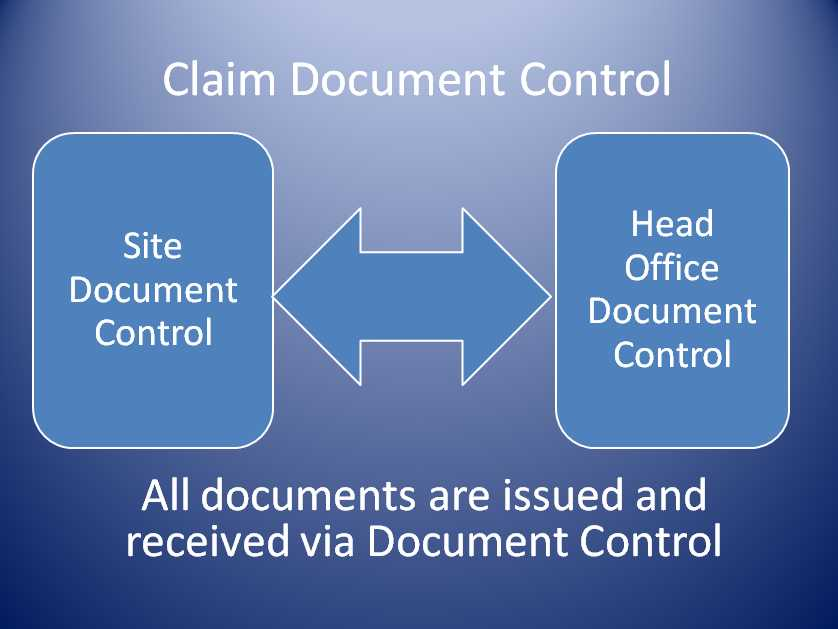
\includegraphics[width=1.3\textwidth]{./graphics/document-control-01}
\end{figure}


\section*{Impact of change orders}

The chart below show the impact of change orders and their distribution. 

\begin{figure}
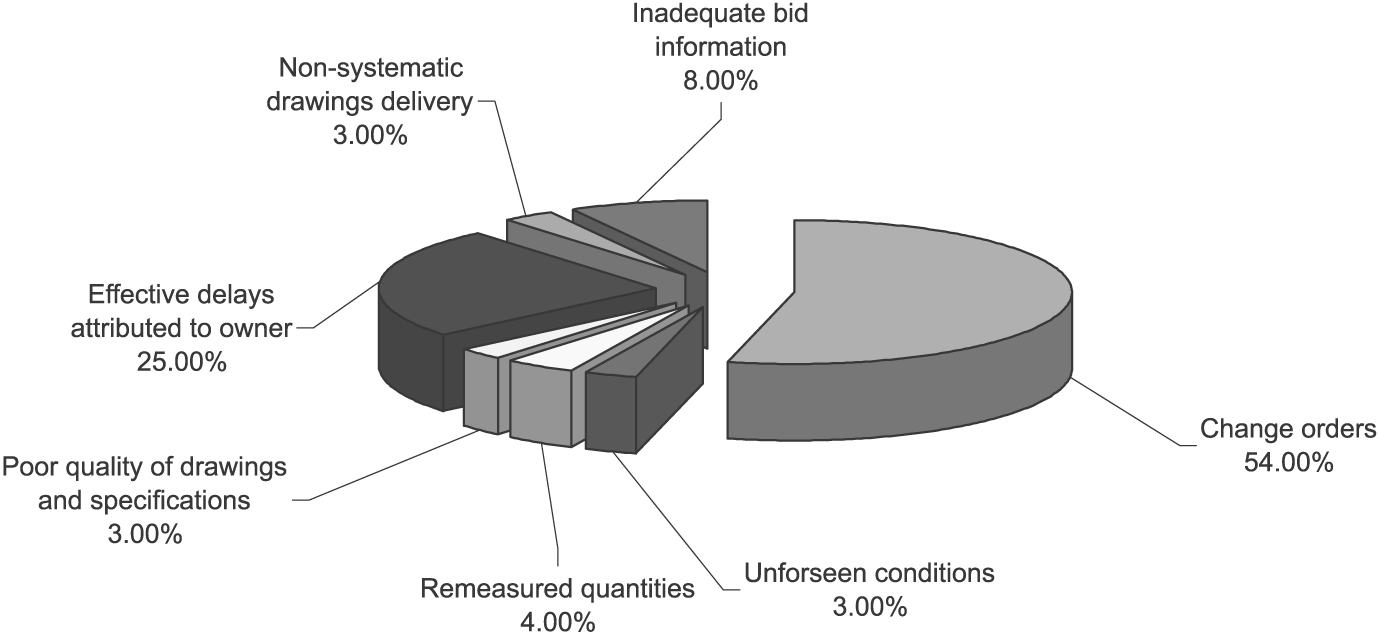
\includegraphics[width=1.3\textwidth]{./graphics/change-orders}
\end{figure}

On Projects where changes are numerous one can produce \textit{measle charts} or
as we call the \textit{chicken pox diagrams}. Like a person afflicted with the
disease your work will be slowed down and the cumulative impact will be much
greater than you think.


\begin{fullwidth}
\begin{figure*}
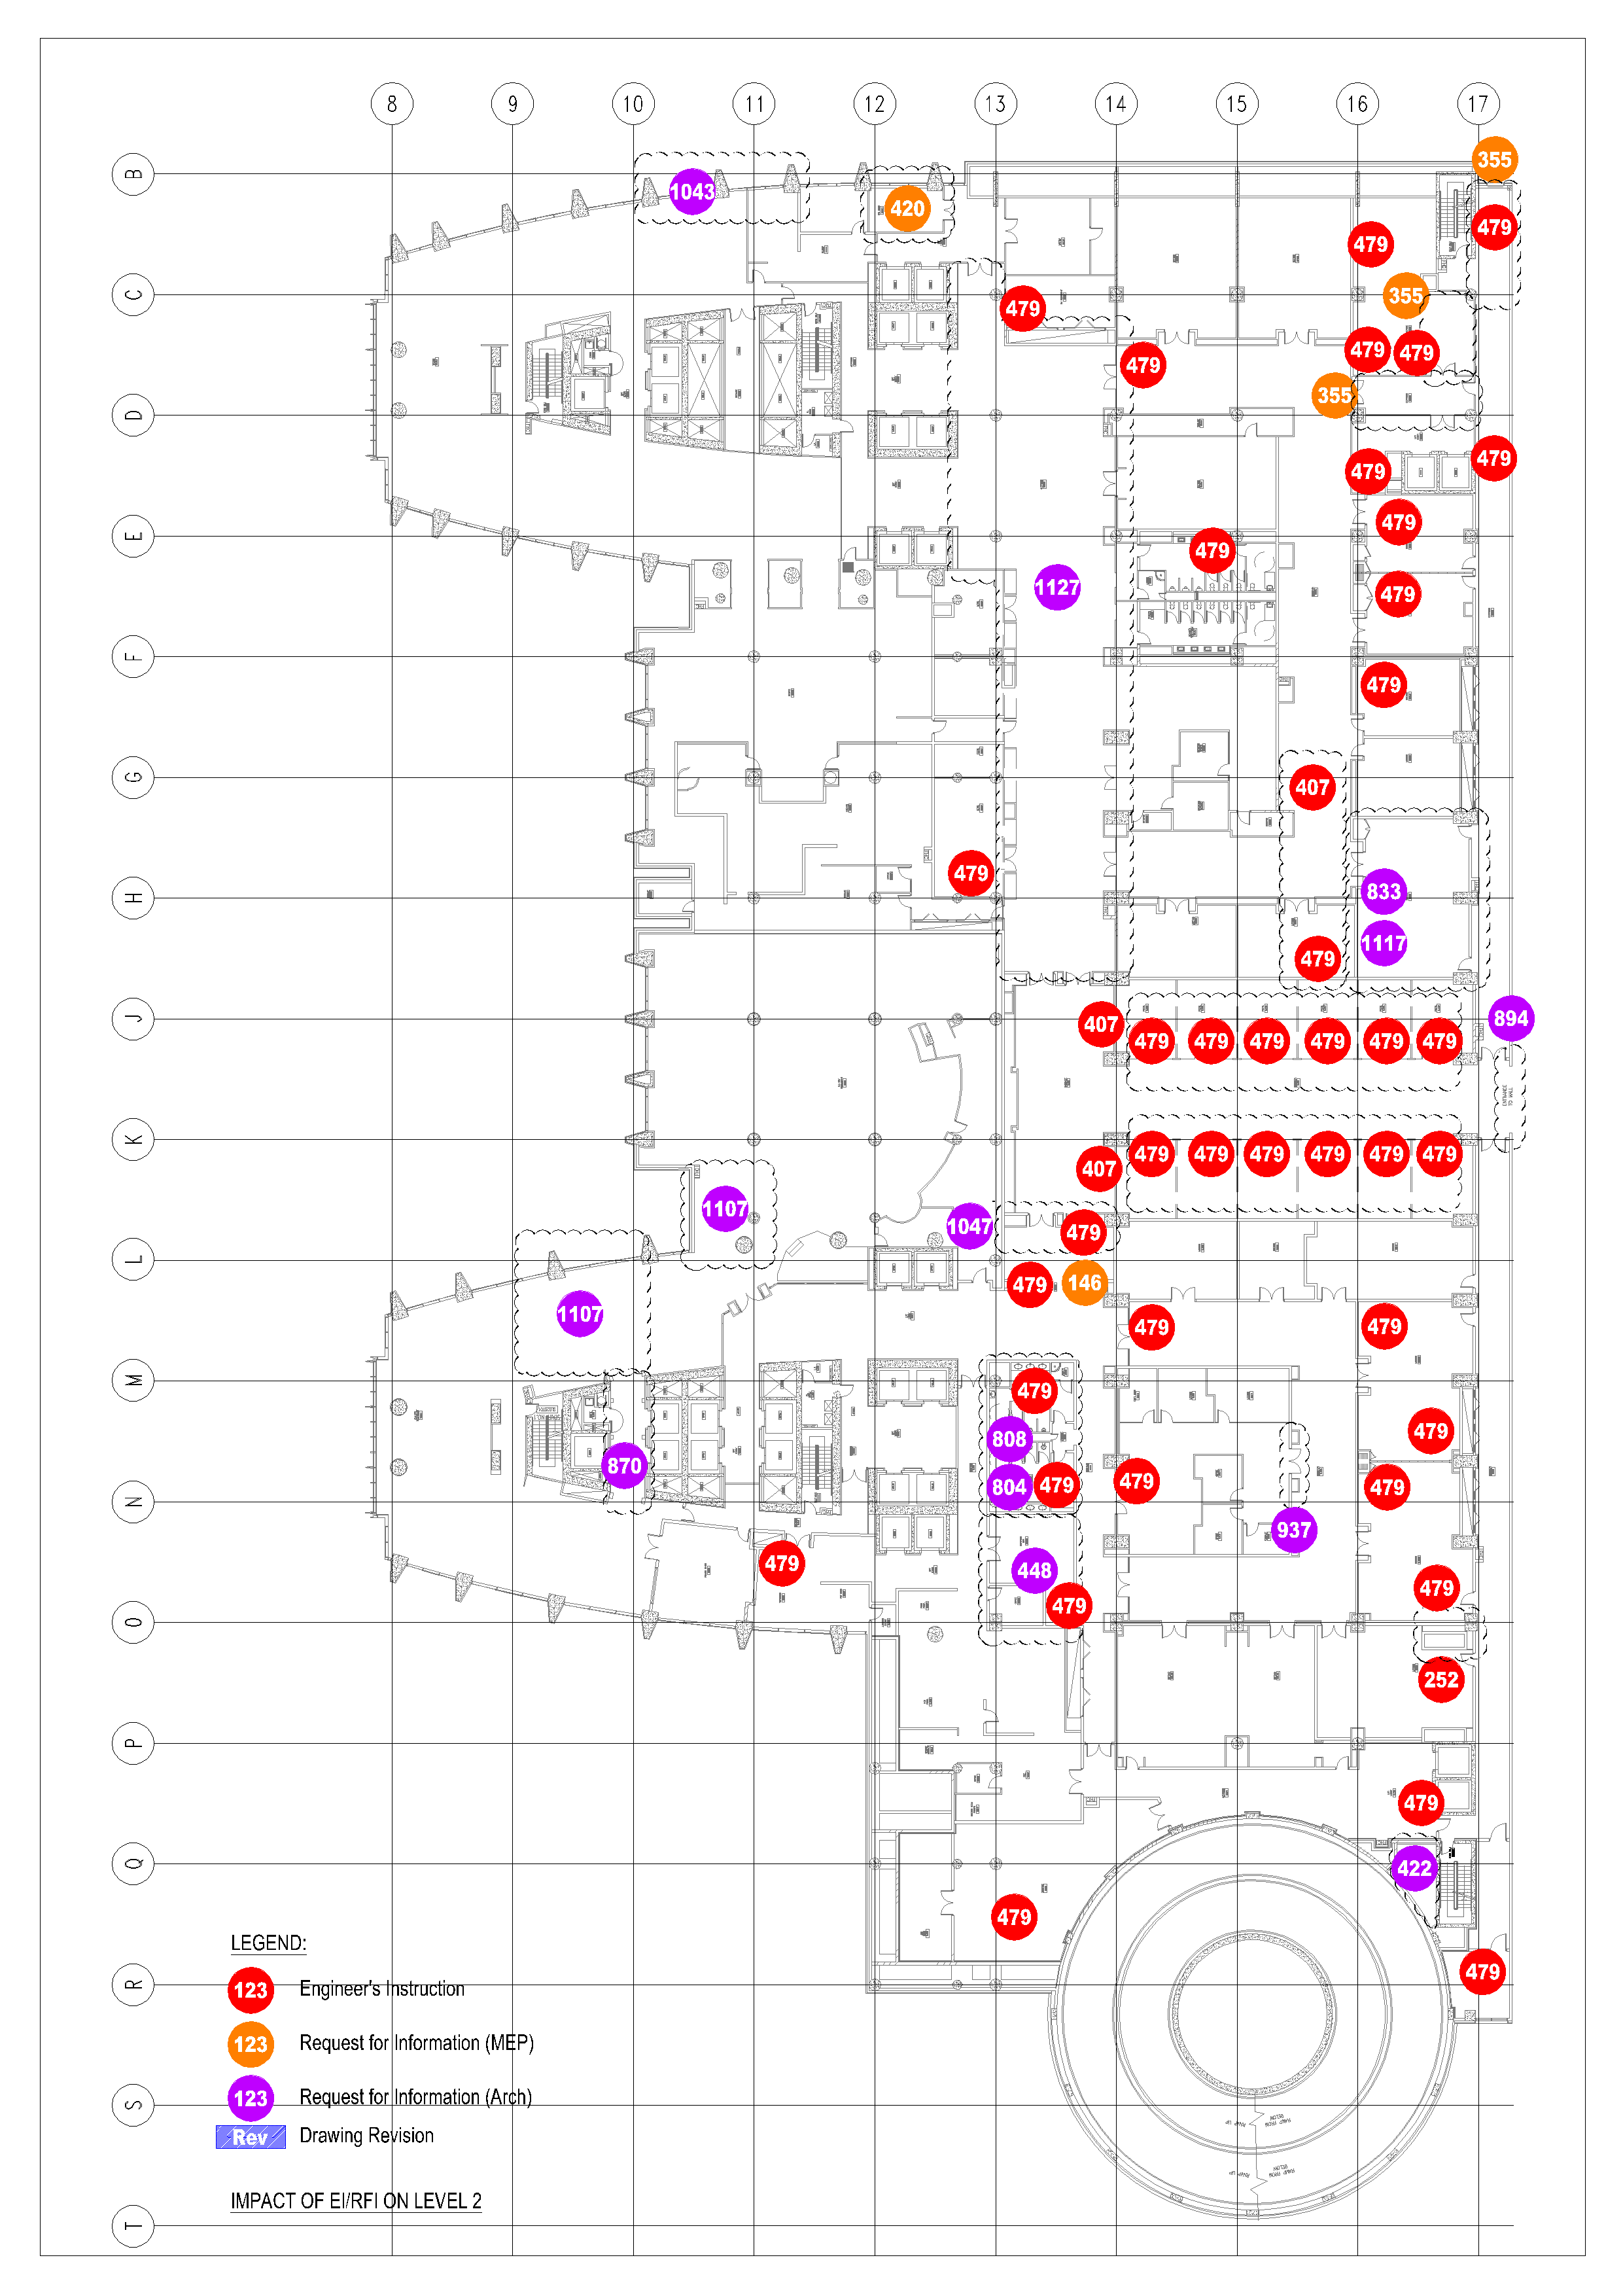
\includegraphics[width=1.1\textwidth]{./graphics/AHU/cpL2}
\caption{Chicken pox diagram showing effect of EIs and major RFIs on Level 2.}
\end{figure*}
\end{fullwidth}

\section*{Recording the changes}

Once a Change Order is initiated a number of steps need to be taken
to ensure that contemporaneous records are kept.

The Site QS needs to ensure that a letter is dispatched recording the fact
that the change order will have a time and a cost impact.

The Engineering Manager will need to ensure that the Change Order is reflected
permanently on drawings. The Shop Drawings need to be revised. Please ensure
that revision clouds are included and that the revision text clearly states
the reason for the change.

The Project Manager and Section Engineers will need to assess the impact of
the EI and inform the Commercial Manager of the impact.

The QS will produce weekly and monthly reports as well as record on the
monthly valuations the impact.

\begin{fullwidth}
\begin{table}[htbp]
\vspace{1cm}
\small
\begin{tabular}{l c c c c c c c c c c c c c c c c c c c}
\toprule
~ &Dec & Jan & Feb & Mar & Apr& May & Jun & Jul & Aug & Sep &Oct & Nov &Dec &Jan & Feb  & Total\\
~ &09  & 10  & 10  & 10  & 10 & 10  & 10  & 10  & 10  & 10  &10  & 10   &10 &11&11&11 \\
\midrule
Phase 3a &17 &9 &10 &17 &9 &21 &12 &15 &16 &13 &15 &15 &7 &6&6&187\\
Phase 3b &1   &3 &0 &3 &2 &5 &0 &3 &3 &1 &3 &11 &4 &6&nil&46\\
\midrule
Phase 2a$+$3b &18 &12 &10 &20 &11 &26 &12 &18 &19 &14 &18 &26 &11 &12&16&233\\

\bottomrule
\end{tabular}
\hskip-10cm\caption{Total number of EIs received since the MOU}
\label{tbl:EI}
\end{table}
\end{fullwidth}

\begin{fullwidth}
\begin{table}[htbp]
\vspace{1cm}
\small
\begin{tabular}{l c c c c c c c c c c c c c c c c c c c}
\toprule
~ &Dec & Jan & Feb & Mar & Apr& May & Jun & Jul & Aug & Sep &Oct & Nov  & Dec & Jan & Feb & Total\\
~ &09  & 10  & 10  & 10  & 10 & 10  & 10  & 10  & 10  & 10  &10  & 10   &10 &11 & 11& 11\\
\midrule
Phase 3a &34  & 38  & 63  & 51  & 56 & 50  & 51  & 79  & 32  & 36  &32  & 41   &31&38&17&661 \\
Phase 3b &12 &19 &12 &7 &28 &24 &23 &21 &5 &8 &12 &13 &5&6&7&204\\
\midrule
Phase 2a$+$3b &46 &57 &75 &58 &84 &74 &74 &100 &37 &44 &44 &54 &36&44&24&865\\

\bottomrule
\end{tabular}
\caption{Total number of RFIs issued since the MOU}
\label{tbl:RFI}
\end{table}
\end{fullwidth}


Charts can assist to better visualize problems with Engineer's Instructions
and RFIs.

\chapter{Cumulative Impact of other EIs and RFIs}
\newthought{A growing list of Engineer's Instructions and Requests for Information} followed-up, the signing of the Memorandum of Agreement. The growth of the EIs is shown graphically in Figure~\ref{EIplots}. As at the end of May 2011, there were 300 EIs issued and 1054 RFIs.
Not only the Engineer failed to complete his design by the 15th of December 2009, as agreed with the Contractor and recorded in the Contractor's approved 6.2 Programme of Works, but the Engineer continued with changes well into a year after the planned Completion Date.


\def\monthnames{{"D","J","F","M","A","M","J","J","A","S","O","N","D"}}
\pgfplotsset{width=16cm}

\begin{fullwidth}
\begin{figure*}[htbp]
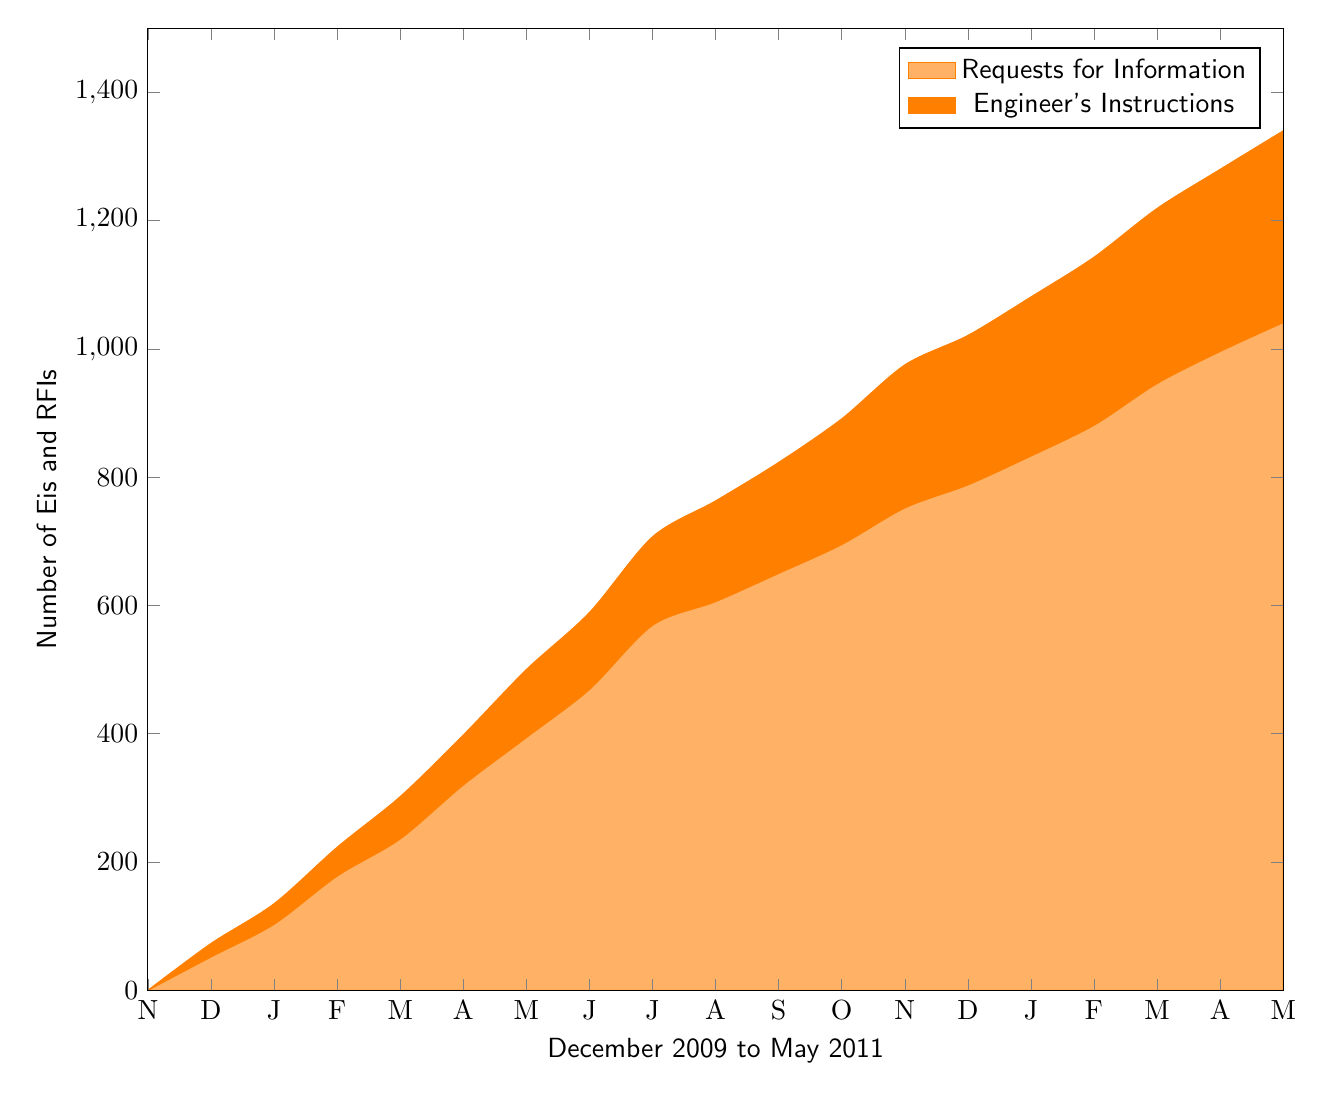
\begin{tikzpicture}
    \begin{axis}[
        smooth,
        stack plots=y,
        area style,
        enlarge x limits=false,
        ymin=0,ymax=1500,
        xlabel=\textsf{December  2009 to May 2011},
        ylabel=\textsf{Number of Eis and RFIs},
        xtick=data,
        %no need to repeat months more than a year
        xticklabel={\pgfmathparse{\monthnames[Mod(\tick-1,12)]}\pgfmathresult}]
\addplot[color=orange,fill=orange!60] coordinates
		{(0,0) (1,52) (2,103) (3,178) (4,236) (5,320) (6,394)%
                (7,469) (8,569) (9,606) (10,650) (11,695) (12,752)%
                (13,788) (14,833)  (15,881) (16,946) (17,996) (18,1041)
               } 
		\closedcycle;
	\addplot[color=orange,fill=orange] coordinates
		{(0,0) (1,21) (2,32) (3,45) (4,66) (5,78) (6,106)%
                (7,120) (8,138) (9,157) (10,173) (11, 196) (12,223)%
               (13,233) (14,248) (15,262) (16,273) (17,284) (18,299)
               }
		\closedcycle;
    \addlegendentry{\textsf{Requests for Information}}
    \addlegendentry{\textsf{Engineer's Instructions}}
    
   
 
    \end{axis}
\end{tikzpicture}
\caption{Plots showing the growth of Engineer's Instructions and their relationship to Requests for Information, the relationship can be observed clearly. See for example the \textit{bumps} at around April-May 2010.}
\label{EIplots}
\end{figure*}
\end{fullwidth}

No Project, where the Design is incomplete can be completed. It is obvious neither the Owner that could instruct the Engineer to add resources to his Team, nor the Engineer considered the Completion Date to be of \textit{essence}.

The Contractor on its part, accelerated works in sections that were critical for the Owners Direct Contractor to have access, providing this access at the end of June 2010.

% start tikzpicture,define styles
% define a style called activity
\tikzstyle{activity}=[draw,
                      rectangle,
                      rounded corners, 
                      fill=black!5,
                      thick,
                      minimum width=2.9cm,
                      minimum height=2.2cm, 
                      text width=2.5cm
                      ]
\begin{figure*}
\begin{tikzpicture}[mystylei/.style={draw,ellipse,rounded corners, fill=gray!23,thick,minimum
width=3cm,minimum height=1cm, text width=2.5cm, text centered}]


%start to define nodes relative to each other
\newcommand\addblock[2]{\node[activity, node distance=0] (#1) {\textsc{\textbf{#1}}. \textsf{#2}};\def\temp{#1}}

\def\addblockbelow#1#2{\node[activity] (#1) [below=of \temp] {#1. \textsf{#2}};\draw[->] (\temp) -- (#1);
\def\temp{#1}
}

\addblock{1}{Mark EI or RFI implications on drawings}
\addblockbelow{B}{EM to identify implications}
\addblockbelow{C}{Issue Impact form to CM}
\addblockbelow{D}{Obtains approval for revisions. iterates if necessary.}
\addblockbelow{5}{Obtains approval for revisions. iterates if necessary.}


%%\node[activity] (C) [below=of B] {C. Issue Impact form to CM}; 
%\node[activity] (D) [below=of C] {D. Obtains approval for revisions. iterates if necessary.};

%second column with a bit of a distance
\node[activity,node distance=1.3cm] (E) [right=of 1] {E. Commercial Manager, reviews};  
\node[activity,node distance=1.3cm] (F) [right=of B] {F. Impact Forms};
\node[activity,node distance=1.3cm] (G) [right=of C] {G. issue claim}; 

%% Third column      
\node[activity,node distance=1.3cm] (H)  [right=of E] {H. PM reviews}; 
\node[activity, node distance=1.3cm] (J) [right=of D] {J. Cause, narrative};

\node[activity,node distance=1.3cm] (H1) [right=of F] {H1. Plans the works. Issues stop orders if necessary};

%empty node for the gap in column 2 row 3
  
\node[activity,node distance=1.3cm] (K) [right=of G] {K. Issue Impact Form to CM. Photographic records and a lot of other stuff in the meanime};       
\node[activity,node distance=1.3cm] (H2) [right=of J] {H2. Arranges materials and installation (WIR)}; 



%connect the nodes
%\draw[->] (1) -- (B);
%\draw[->] (B) -- (C);
%\draw[->] (C) -- (D);
\draw[->] (E) -- (F);
\draw[->] (F) -- (G);
\draw[->] (G) -- (J);
\draw[->] (C) to [out=360,in=180] (F);
\draw[->] (D) to [out=360,in=199] (F);
\draw[->] (K) to [out=180,in=360] (F);
\draw[->] (H1)-- (K);
\draw[->] (H) -- (H1);
\draw[->] (K) -- (H2);
%\draw[->] (C) -- (K);

\end{tikzpicture}
\caption{Workflow for Engineers Instructions and RFI works. All Departments get involved when there is a Change Order. Evaluate Change Orders as they occur and keep contemporaneous records. }
\end{figure*}






































